\documentclass[a4paper]{article}
\usepackage[utf8]{inputenc}
\usepackage[MeX]{polski}
\usepackage{amsmath}
\usepackage{amssymb}
\usepackage{float}
\usepackage{natbib}
\usepackage{graphicx}
\usepackage{listings}
\usepackage[euler]{textgreek}
\usepackage{nowidow}
\usepackage{subfiles}
\usepackage{geometry}
\usepackage{makecell}
\usepackage{ragged2e}
\usepackage{wrapfig}
\usepackage{subfig}
\usepackage{multicol}
\usepackage[export]{adjustbox}
\usepackage{xcolor}
\usepackage{blindtext}
\usepackage{hyperref}

\begin{document}

\begin{titlepage}
    \begin{center}
        \vspace*{1cm}
            
        \Huge
        \textbf{UMIR}
            
        \vspace{0.5cm}
        \LARGE
        Raport z projektu "zdjęcia dronów"
            
        \vspace{1.5cm}
            
        Zespół 8:\\
        \textbf{Kazimierz Roman\\
                Artur Romaniuk\\
                Karol Duszczyk}
            
        \vfill

        \vspace{0.8cm}
            
        \Large
        \today
        
            
    \end{center}
\end{titlepage}

\tableofcontents

\newpage

\section{Dane}
\subsection{Dataset}
W projekcie użyliśmy zbioru zdjęć \href{https://www.kaggle.com/datasets/cybersimar08/drone-detection}{\textit{Drone Detection}}. Zbiór ten zawiera 4 klasy: 0 - samolot, 1 - dron, 2 - helikopter, 3 - ptak.

\subsection{Data augmentation}

W każdym zadaniu zastosowano augmentację danych. Zastosowano następujące transformacje:
\begin{itemize}
    \item Random Rotation - obrót o losowy kąt z zakresu $(-54^{\circ} , +54^{\circ})$ (factor=0.15)
    \item Random Translation - przesunięcie o losową wartość z zakresu $(-10\%, +10\%)$ (height\_factor=0.1, width\_factor=0.1)
    \item Random Flip - losowe odbicie w poziomie lub pionie
    \item Random Contrast - losowa zmiana kontrastu z zakresu $(-10\%, +10\%)$ (factor=0.1)
\end{itemize}


\section{Zadanie 1: Uczenie klasyfikatora}
\section{Zadanie 1 - Uczenie klasyfikatora}

\subsection{Opis zadania}
Celem tego zadania było wykorzystanie wstępnie wytrenowanej sieci do uczenia wyłącznie części klasyfikującej (ostatnich warstw o połączeniach kompletnych). Następnie wyniki klasyfikacji zostały przeanalizowane. Kolejnym krokiem było zastąpienie części klasyfikującej sieci klasyfikatorem SVM z różnymi jądrami: liniowym, kwadratowym (poly) oraz RBF. Wyniki klasyfikacji dla każdego jądra zostały porównane, a szczególna uwaga została poświęcona efektowi dopuszczenia błędnych klasyfikacji.

\subsection{Wybór architektury modelu}
Do realizacji zadania wykorzystano sieć EfficientNetB0, wstępnie wytrenowaną na zbiorze ImageNet. Warstwy bazowe modelu zostały zamrożone, aby nie były aktualizowane podczas uczenia. Ostatnie warstwy klasyfikujące zostały zastąpione następującą strukturą:
\begin{itemize}
    \item Warstwa GlobalAveragePooling2D,
    \item Warstwa Dropout (z prawdopodobieństwem $0.2$),
    \item Warstwa Dense z liczbą neuronów odpowiadającą liczbie klas i funkcją aktywacji softmax.
\end{itemize}

\noindent Struktura modelu została przedstawiona w Tabeli~\ref{tab:model_summary}.
\begin{table}[h!]
\centering
\begin{tabular}{|l|l|l|}
\hline
\textbf{Warstwa}                  & \textbf{Rozmiar wyjścia}       & \textbf{Liczba parametrów} \\ \hline
Wejście                          & (None, 224, 224, 3)           & 0                          \\ \hline
EfficientNetB0                   & (None, 7, 7, 1280)            & 4,049,571                  \\ \hline
GlobalAveragePooling2D           & (None, 1280)                  & 0                          \\ \hline
Dropout                          & (None, 1280)                  & 0                          \\ \hline
Dense                            & (None, 4)                     & 5,124                      \\ \hline
\end{tabular}
\caption{Podsumowanie modelu klasyfikatora.}
\label{tab:model_summary}
\end{table}

\subsection{Wyniki uczenia klasyfikatora}
Wyniki procesu uczenia, przedstawione na wykresach (Rys.~\ref{fig:loss_accuracy}), ilustrują zmniejszanie się wartości funkcji straty (loss) oraz wzrost dokładności (accuracy) w zbiorach treningowym i walidacyjnym.

\begin{figure}[h!]
    \centering
    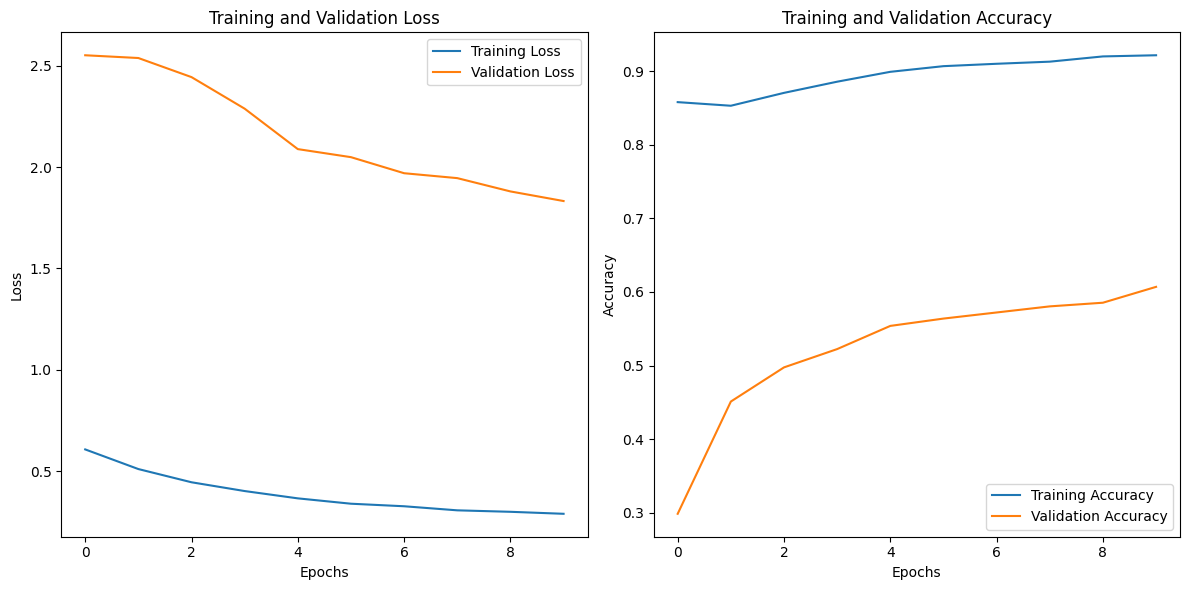
\includegraphics[width=0.9\textwidth]{loss.png}
    \caption{Wykresy funkcji straty i dokładności dla zbiorów treningowego i walidacyjnego.}
    \label{fig:loss_accuracy}
\end{figure}

\begin{table}[h!]
\centering
\begin{tabular}{|c|c|c|c|c|}
\hline
\textbf{} & \textbf{Klasa 0} & \textbf{Klasa 1} & \textbf{Klasa 2} & \textbf{Klasa 3} \\ \hline
\textbf{Klasa 0} & 41 & 39 & 46 & 2 \\ \hline
\textbf{Klasa 1} & 26 & 206 & 2 & 0 \\ \hline
\textbf{Klasa 2} & 4 & 7 & 97 & 3 \\ \hline
\textbf{Klasa 3} & 29 & 51 & 32 & 11 \\ \hline
\end{tabular}
\caption{Macierz pomyłek dla zbioru testowego.}
\label{tab:confusion_matrix_last_layer}
\end{table}

\subsection{Zastąpienie klasyfikatora sieci SVM}
W celu poprawy klasyfikacji, cechy wyodrębnione z ostatniej warstwy modelu EfficientNetB0 zostały wykorzystane do uczenia klasyfikatora SVM z różnymi jądrami. Wyniki klasyfikacji zostały ocenione za pomocą miar takich jak precision, recall i F1-score.

\subsubsection{Wyniki dla różnych jąder}
\begin{itemize}
    \item \textbf{Jądro liniowe:} Dokładność wyniosła $88\%$, a F1-score dla poszczególnych klas mieściło się w zakresie $0.80$--$0.95$. 
    \item \textbf{Jądro kwadratowe (poly):} Najwyższa dokładność na poziomie $93\%$, przy wysokich wartościach precision i recall.
    \item \textbf{Jądro RBF:} Dokładność również wyniosła $93\%$, jednak efektywność była różna w zależności od klasy.
\end{itemize}

\subsubsection{Macierze pomyłek}
Macierze pomyłek dla każdego jądra pozwoliły na identyfikację klas trudniejszych do rozróżnienia, co przedstawiono w poniższym przykładzie dla jądra liniowego (Tabela~\ref{tab:confusion_matrix_linear}).
\begin{figure}[h!]
    \centering
    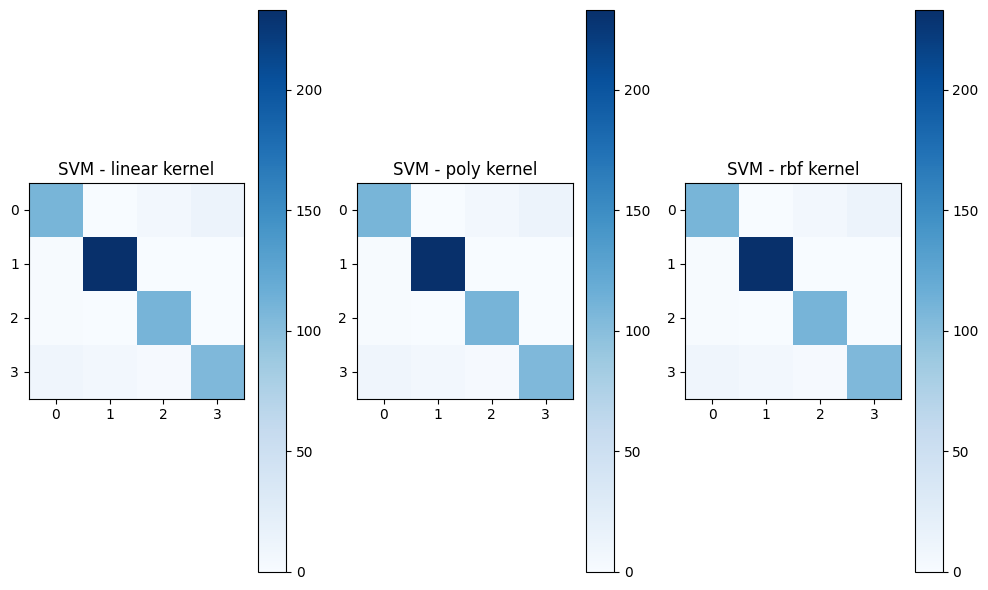
\includegraphics[width=0.9\textwidth]{svm.png}
    \caption{Wykresy funkcji straty i dokładności dla zbiorów treningowego i walidacyjnego.}
    \label{fig:loss_accuracy}
\end{figure}

\subsection{Podsumowanie}
Porównanie wyników klasyfikacji dla różnych jąder SVM wykazało, że jądra kwadratowe i RBF osiągają wyższą dokładność niż jądro liniowe, co sugeruje lepsze odwzorowanie granic decyzyjnych w bardziej złożonych przestrzeniach. Wyniki te wskazują na możliwość dalszej poprawy wydajności modelu poprzez dostrojenie hiperparametrów klasyfikatora.


\section{Zadanie 2: Uczenie sieci głębokiej}
\subsection{Przeprowadzić uczenie ostatniej warstwy splotowej wraz z częścią
klasyfikującą}

Ostatnią warstwą splotową w sieci EfficientNetB0 jest warstwa top\_conv, która jest trzecią warstwą od góry. Z tego powodu zamrożono wszystkie warstwy sieci poza trzema ostatnimi. Jako wagi początkowe zastosowano wagi imagenet. Następnie przeprowadzono uczenie z wykorzystaniem zbioru treningowego. W trakcie uczenia zastosowano optymalizator Adam, funkcję straty sparse categorical crossentropy oraz metrykę accuracy. Przetestowano różne wartości współczynnika uczenia, ostatecznie wybrano wartość 1e-5. Po 40 epokach uczenia osiągnięto na zbiorze testowym \textbf{accuracy na poziomie 0.74, loss na poziomie 0.66} oraz macierz pomyłek przedstawioną w tabeli \ref{tab:z2a}. Wyniki uczenia w czasie przedstawiono na rysunku \ref{fig:z2a}. Dalsze uczenie nie przynosiło poprawy wyników.

% Confusion Matrix:
%  [[ 32  18  29  49]
%  [  0 229   4   1]
%  [  1   4 105   1]
%  [  4  19  24  76]]

\begin{table}[H]
\centering
\begin{tabular}{|c|c|c|c|c|}
\hline
klasa & 0 & 1 & 2 & 3 \\ \hline
0 & 32 & 18 & 29 & 49 \\ \hline
1 & 0 & 229 & 4 & 1 \\ \hline
2 & 1 & 4 & 105 & 1 \\ \hline
3 & 4 & 19 & 24 & 76 \\ \hline
\end{tabular}
\caption{Macierz pomyłek dla zadania 2a}
\label{tab:z2a}
\end{table}

\begin{figure}[H]
    \centering
    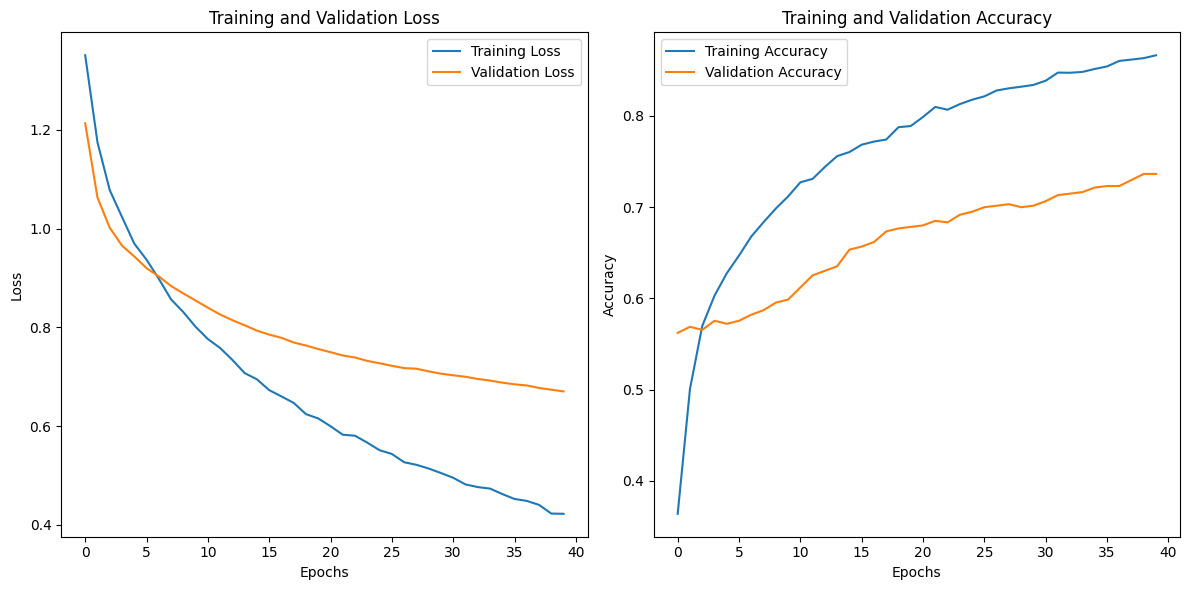
\includegraphics[width=0.8\textwidth]{img/z2a.png}
    \caption{Wyniki uczenia dla zadania 2a}
    \label{fig:z2a}
\end{figure}




%ile parametrów trainable

\subsection{Wytrenować całą sieć dla zadanych danych}
W tym zadaniu odmrożono wszystkie warstwy EfficientNetB0 i nadano im wagi początkowe imagenet. Następnie przeprowadzono uczenie z wykorzystaniem zbioru treningowego. W trakcie uczenia zastosowano optymalizator Adam, funkcję straty sparse categorical crossentropy oraz metrykę accuracy. Przetestowano różne wartości współczynnika uczenia, ostatecznie wybrano wartość 1e-5. Podczas uczenia zastosowano mechanizm early stopping, który zatrzymywał uczenie jeśli przez 4 epoki nie następowała poprawa wyników. Uczenie zatrzymało się po 22 epokach. Ostatecznie osiągnięto na zbiorze testowym \textbf{accuracy na poziomie 0.63, loss na poziomie 1.01} oraz macierz pomyłek przedstawioną w tabeli \ref{tab:z2b}. Wyniki uczenia w czasie przedstawiono na rysunku \ref{fig:z2b_with_w}.

% Test loss: 1.0159192085266113, Test accuracy: 0.6325503587722778
% Confusion Matrix:
%  [[ 56  17  55   0]
%  [  0 234   0   0]
%  [ 22   1  87   1]
%  [  9  36  78   0]]

\begin{table}[H]
\centering
\begin{tabular}{|c|c|c|c|c|}
\hline
klasa  & 0 & 1 & 2 & 3 \\ \hline
0 & 56 & 17 & 55 & 0 \\ \hline
1 & 0 & 234 & 0 & 0 \\ \hline
2 & 22 & 1 & 87 & 1 \\ \hline
3 & 9 & 36 & 78 & 0 \\ \hline
\end{tabular}
\caption{Macierz pomyłek dla zadania 2b z wagami imagenet}
\label{tab:z2b}
\end{table}
    
\begin{figure}[H]
    \centering
    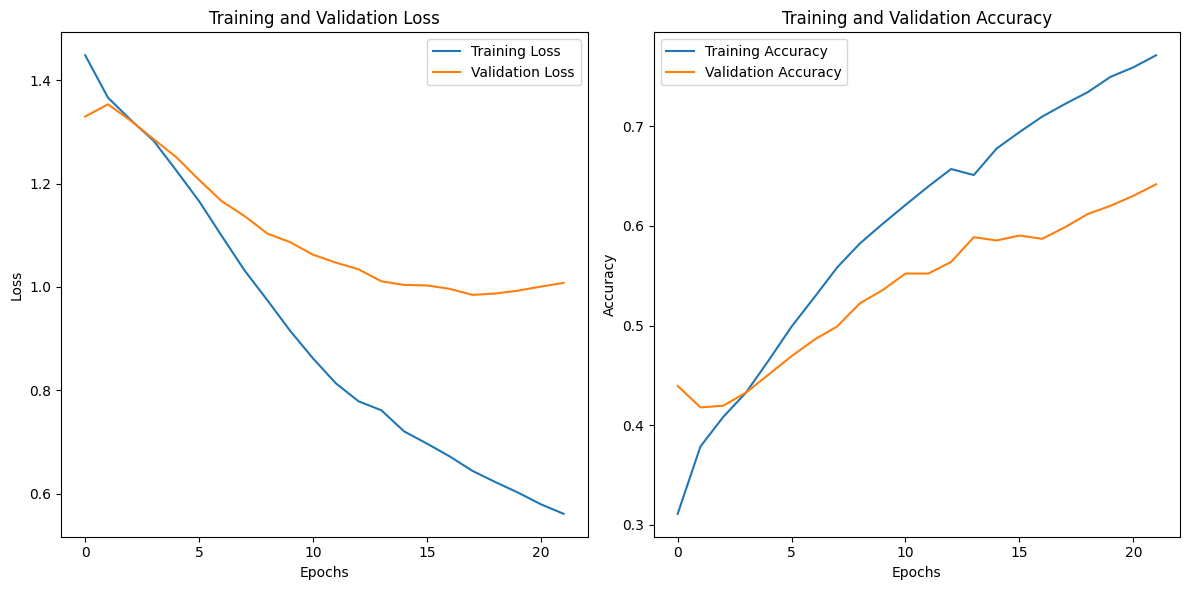
\includegraphics[width=0.8\textwidth]{img/z2b_with_w.png}
    \caption{Wyniki uczenia dla zadania 2b z wagami imagenet}
    \label{fig:z2b_with_w}
\end{figure}

Próbowano także wytrenować całą sieć bez zadanych wag początkowych, jednak w tym przypadku wyniki były dużo gorsze (accuracy na poziomie 0.38). Może to wynikać z faktu, że zbiór treningowy jest stosunkowo mały, a wagi początkowe z imagenet są lepsze niż losowe.

\subsection{Uprościć strukturę sieci wytrenowanej w zadaniu 2c (np. poprzez
usunięcie jednej lub więcej końcowych warstw splotowych, usunięcie
warstw regularyzujących itp.) i ponowić uczenie}

\subsection{Zanalizować wyniki 2 abc}

\section{Zadanie 3: Wizualizacja}

\label{sec:z3}

Celem zadania trzeciego było wykonanie wszechstronnej wizualizacji i interpretacji wyników działania sieci głębokich (oraz klasyfikatorów wykorzystujących ich cechy). W~szczególności zrealizowano następujące etapy:
\begin{enumerate}
    \item \textbf{Analiza błędnych klasyfikacji (misclassifications)} -- identyfikacja i omówienie przypadków, w których model się myli, oraz wskazanie możliwych przyczyn błędów.
    \item \textbf{Wizualizacja obszarów uwagi (CAM, Class Activation Map)} -- sprawdzenie, które fragmenty obrazu mają największy wpływ na odpowiedź modelu.
    \item \textbf{Wizualizacja wewnętrznych warstw (DeepDream)} -- zbadanie i ukazanie sposobu, w jaki wytrenowane filtry sieci reagują na specyficzne wzorce w danych.
    \item \textbf{Testy z własnym zbiorem danych} -- ocena jakości klasyfikatorów na nowym, niestandardowym zbiorze (również generowanym za pomocą \textbf{Fooocus v2.5.0}) oraz prezentacja metryk (Loss, Accuracy, macierze pomyłek, raporty klasyfikacji).
\end{enumerate}

\subsection{Analiza błędnych klasyfikacji}
W~pierwszym kroku dokonano predykcji klas dla wszystkich próbek z~oryginalnego zbioru testowego (zadania 1 i~2), po czym porównano je z rzeczywistymi etykietami. Obrazy sklasyfikowane błędnie zapisywano do osobnego katalogu w celu ich pogłębionej inspekcji (\texttt{misclassified\_images.zip}). 
Przykładowe błędnie sklasyfikowane obrazy dla wersji sieci z klasyfikatorem SVM - jądro poly wraz z etykietami:
\begin{figure}[H]
    \centering
    % Tu wstawić ścieżkę do przykładowego błędnie sklasyfikowanego obrazu
    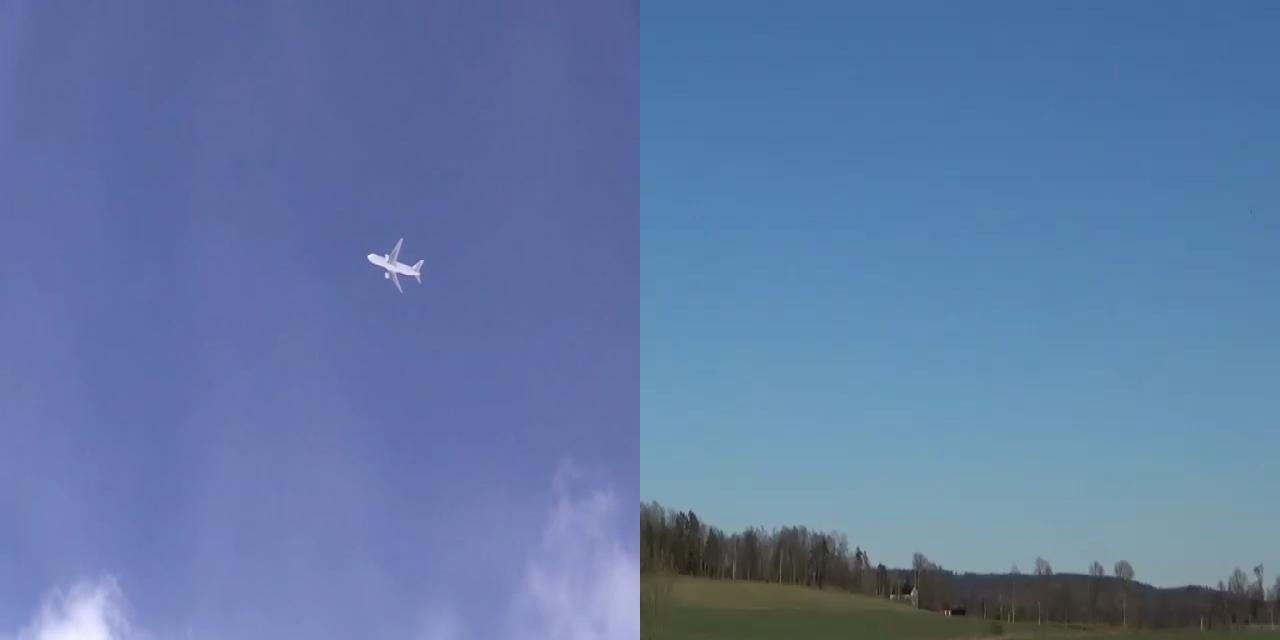
\includegraphics[width=1\textwidth]{img/zad3/bledy.png}
    \caption{ od lewej: [true - samolot (0), predicted - helikopter (2)], [true - ptak (3), predicted - dron (1)]}
    \label{fig:z3_misclass}
\end{figure}

Najczęstsze przyczyny błędów klasyfikacji to:
\begin{itemize}
    \item \textbf{Niska jakość obrazu:} rozmyte lub nieostre zdjęcia, trudne do zinterpretowania nawet przez człowieka,
    \item \textbf{Podobieństwo klas:} daleki dron przypominający ptaka, nietypowy kształt helikoptera z zewnątrz wyglądający jak samolot,
    \item \textbf{Błędy etykiet (label noise):} istniejące w zbiorze przykłady mogą być niepoprawnie oznakowane,
    \item \textbf{Kontekst otoczenia:} sieć bywała zwodzona np.\ przez specyficzne tło (np.\ chmury, budynki).
\end{itemize}


\subsection{Wizualizacja obszarów uwagi (CAM)}
Aby określić, na które regiony obrazu sieć zwraca największą uwagę, wykorzystano technikę \emph{Class Activation Map (CAM)}:
\begin{itemize}
    \item Z~modelu wybrano ostatnią warstwę splotową (\ \texttt{top\_conv} w \emph{EfficientNetB0}),
    \item Wyliczono gradienty od wyniku klasyfikacji do tejże warstwy, a następnie uśredniono (tzw.\ \emph{global average pooling}),
    \item Otrzymaną mapę \emph{heatmap} nałożono na oryginalny obraz (także w wersji zeskalowanej do~128\texttimes128).
\end{itemize}

Dla wytrenowanych wersji sieci z zadania 1,2a,2b,2c wykonano wizualizację obszarów uwagi dla wybranego obrazu testowego (nr 521). Przykładowe wyniki przedstawiono poniżej:

\begin{figure}[H]
    \centering
    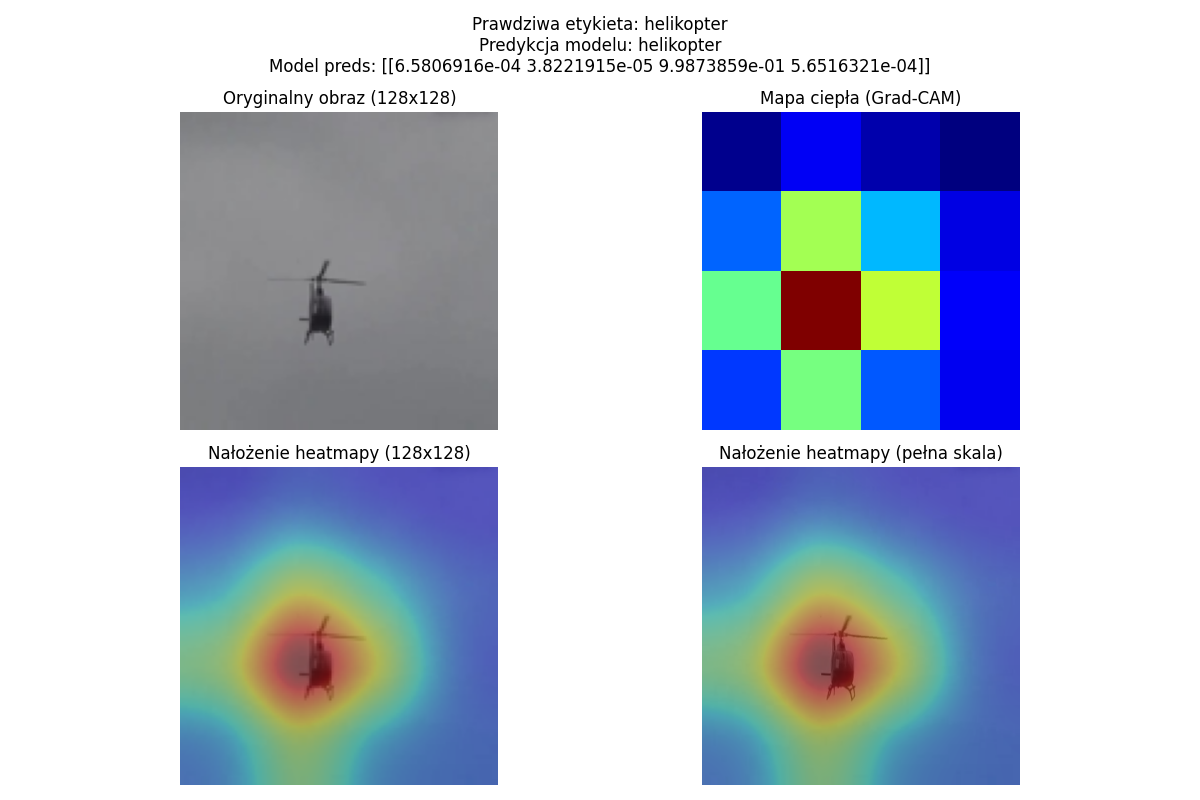
\includegraphics[width=0.9\textwidth]{img/zad3/modelzad1_heatmap_521_true_helikopter_pred_helikopter.png}
    \caption{Przykładowy wynik CAM. Obraz testowy nr. 521 - model z zadania 1 (bez SVM).}
    \label{fig:z3_cam}
\end{figure}
\begin{figure}[H]
    \centering
    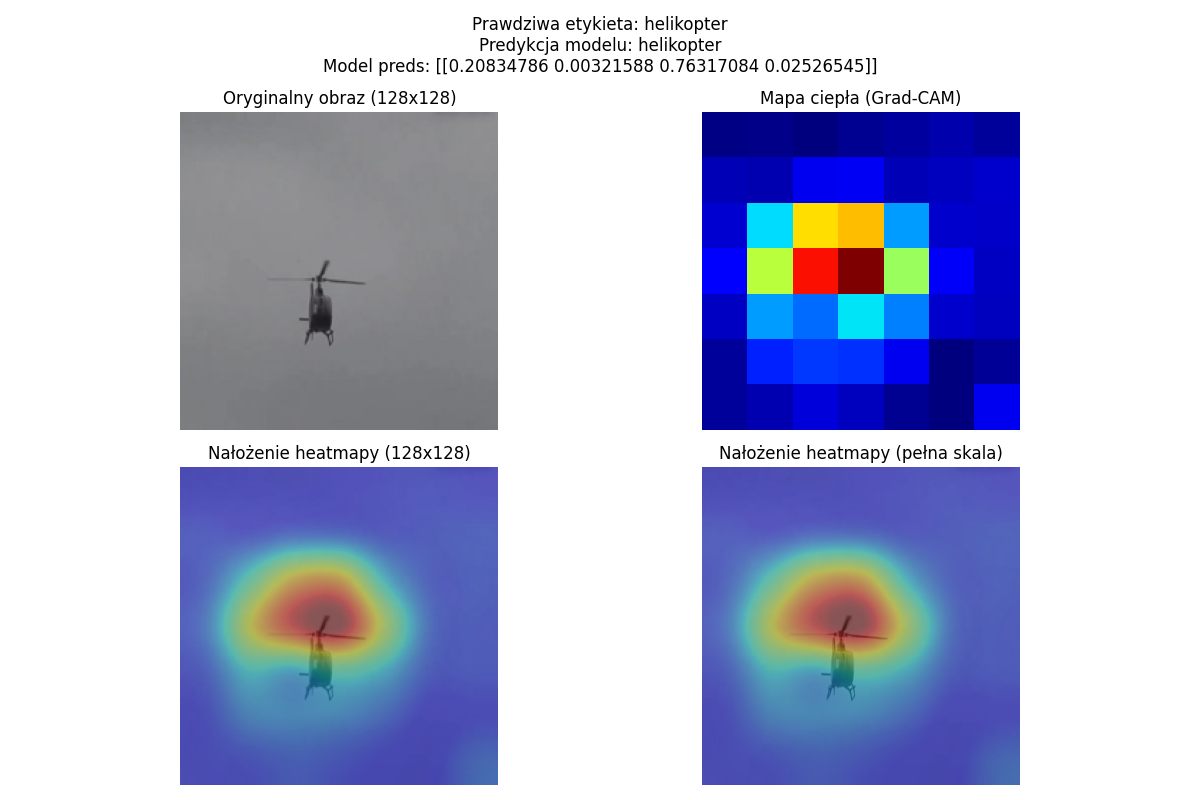
\includegraphics[width=0.9\textwidth]{img/zad3/modelzad2aheatmap_521_true_helikopter_pred_helikopter.png}
    \caption{Przykładowy wynik CAM. Obraz testowy nr. 521 - model z zadania 2a.}
    \label{fig:z3_cam}
\end{figure}
\begin{figure}[H]
    \centering
    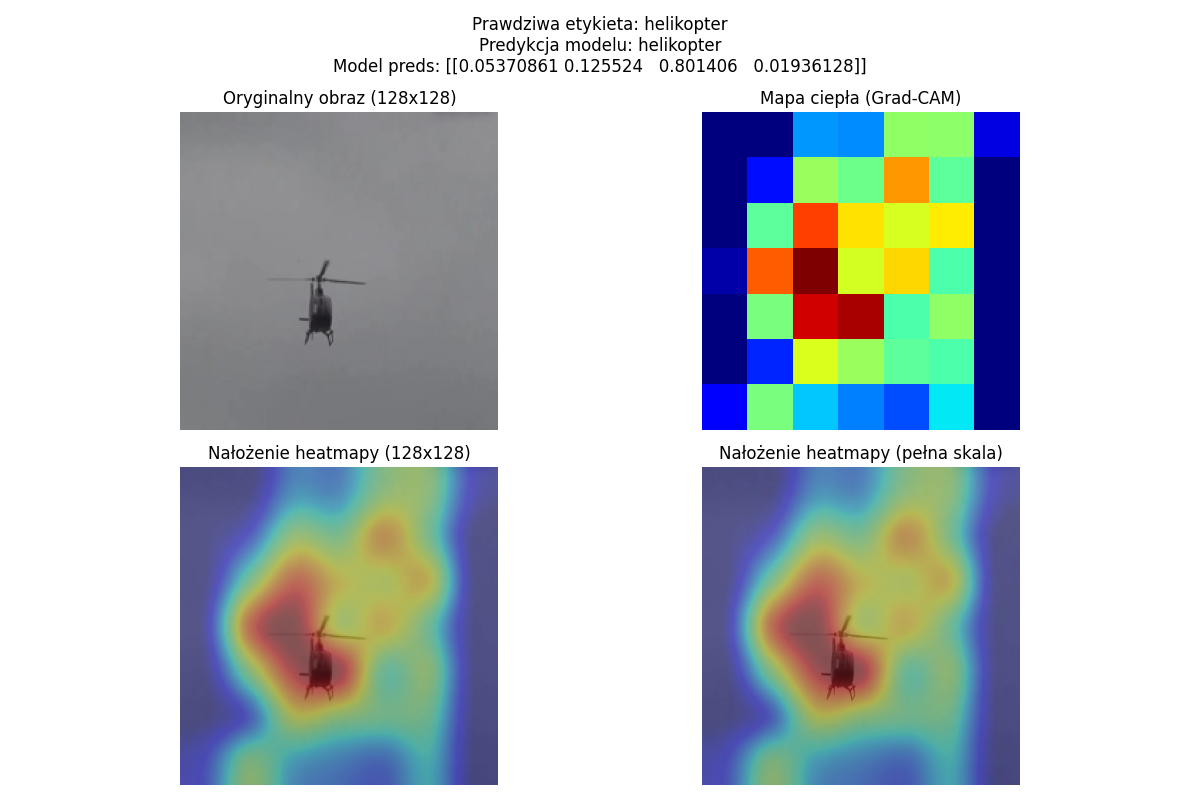
\includegraphics[width=0.9\textwidth]{img/zad3/modelzad2b_heatmap_521_true_helikopter_pred_helikopter.png}
    \caption{Przykładowy wynik CAM. Obraz testowy nr. 521 - model z zadania 2b.}
    \label{fig:z3_cam}
\end{figure}
\begin{figure}[H]
    \centering
    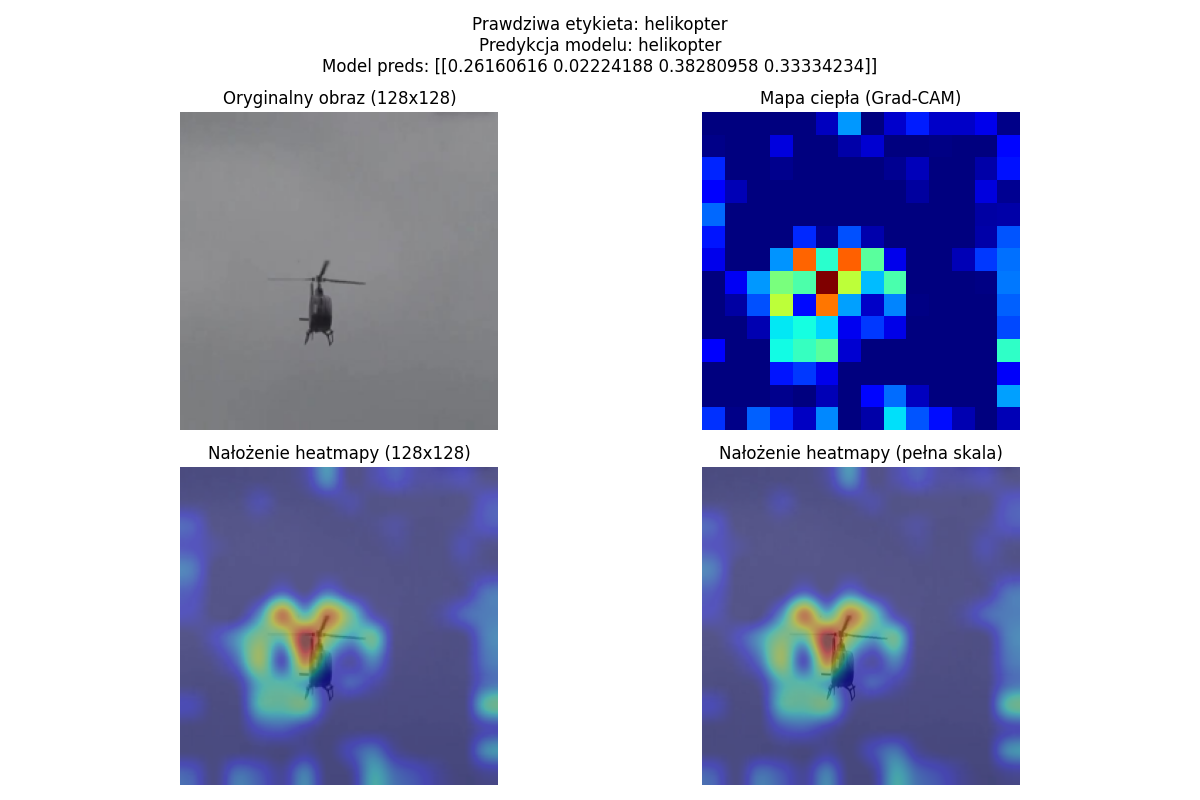
\includegraphics[width=0.9\textwidth]{img/zad3/modelzad2c_heatmap_521_true_helikopter_pred_helikopter.png}
    \caption{Przykładowy wynik CAM. Obraz testowy nr. 521 - model z zadania 2c.}
    \label{fig:z3_cam}
\end{figure}
W prawidłowych klasyfikacjach sieć zwykle koncentruje się na obiekcie (np.\ dronie), natomiast w przypadku błędnych etykiet skupienie może paść na elementy tła i doprowadzić do mylnej decyzji.


\subsection{Wizualizacja wewnętrznych warstw (DeepDream)}
Technika \textbf{DeepDream} umożliwia wizualną eksplorację aktywacji głębszych warstw splotowych:
\begin{itemize}
    \item Dla wybranych warstw (np.\ \texttt{block3a\_activation}, \texttt{block5a\_activation} i \texttt{block7a\_activation} w~\emph{EfficientNetB0}) wykonuje się \emph{gradient ascent} wzmacniający odpowiadające im filtry,
    \item Proces dzieli się na tzw.\ \emph{octave scales}, by uwypuklić różne poziomy szczegółowości (skalowanie w górę obrazu w kolejnych krokach).
\end{itemize}

Wybrany obraz w wersji oryginalnej i po zastosowaniu DeepDream przedstawiono poniżej:
\begin{figure}[H]
    \centering
    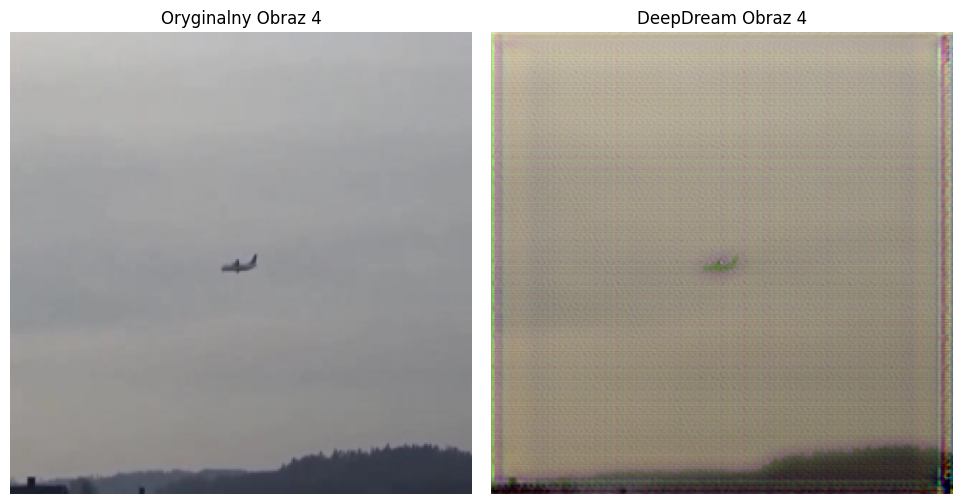
\includegraphics[width=1\textwidth]{img/zad3/deepdream_oryginal.png}
    \caption{Obraz nr. 4 oryginalny (po lewej) i po zastosowaniu DeepDream (po prawej).}
    \label{fig:z3_deepdream}
\end{figure}


Jak widać na Rys.~\ref{fig:z3_deepdream}, sieć „uwydatnia” w obrazie wzory przypominające fraktale i abstrakcyjne tekstury, ujawniając tym samym swoje wewnętrzne detektory krawędzi i wzorców.


\subsection{Testy z własnym zbiorem danych i szczegółowe wyniki}
Aby zbadać uogólnianie modeli na dane odbiegające od oryginalnego podziału \texttt{train/valid/test}, wygenerowano \textbf{160 obrazów} (po~40 dla każdej kategorii: \textit{samolot}, \textit{dron}, \textit{helikopter}, \textit{ptak}) za pomocą programu \textbf{Fooocus v2.5.0}, działającego lokalnie na NVIDIA GeForce GTX\,1070.
Przykładowe obrazy z tego zbioru przedstawiono poniżej:

\begin{figure}[H]
    \centering
    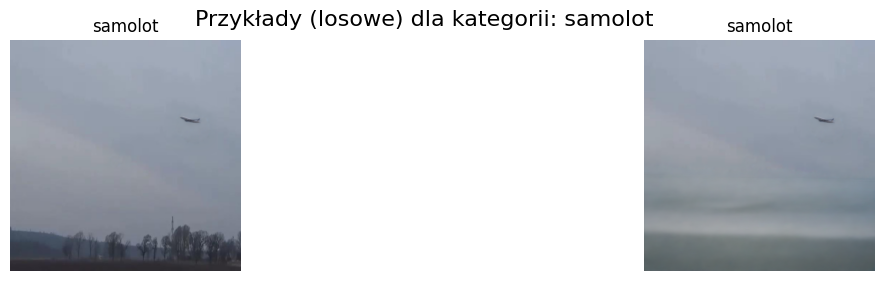
\includegraphics[width=0.95\textwidth]{img/zad3/podpunkt1.png}
    % \caption{Przykładowe obrazy z własnego zbioru danych - kategoria samolot.}
    \label{fig:z3_images}
\end{figure}
\begin{figure}[H]
    \centering
    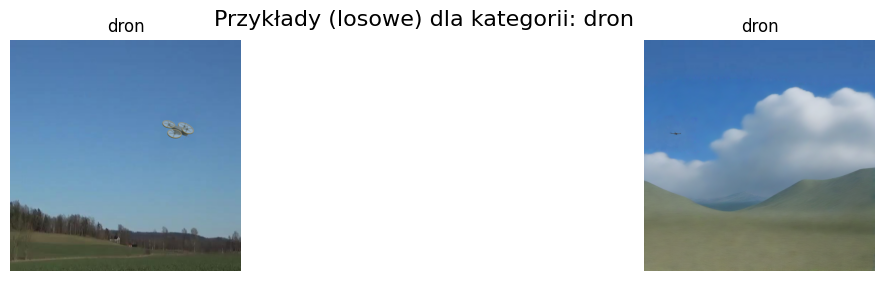
\includegraphics[width=0.95\textwidth]{img/zad3/podpunkt2.png}
    % \caption{Przykładowe obrazy z własnego zbioru danych - kategoria dron.}
    \label{fig:z3_images}
\end{figure}
\begin{figure}[H]
    \centering
    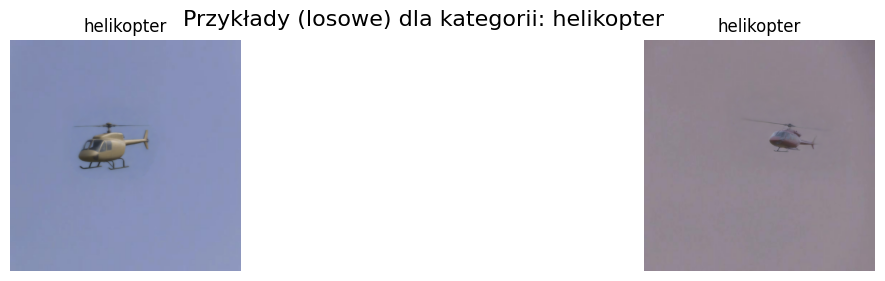
\includegraphics[width=0.95\textwidth]{img/zad3/podpunkt3.png}
    % \caption{Przykładowe obrazy z własnego zbioru danych - kategoria helikopter.}
    \label{fig:z3_images}
\end{figure}
\begin{figure}[H]
    \centering
    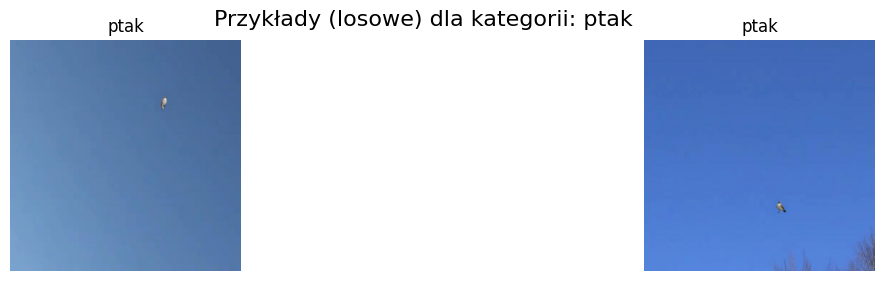
\includegraphics[width=0.95\textwidth]{img/zad3/podpunkt4.png}
    % \caption{Przykładowe obrazy z własnego zbioru danych - kategoria ptak.}
    \label{fig:z3_images}
\end{figure}




Przetestowano cztery finalne modele (z~zadań 1 i 2). Poniżej przedstawiono zestawienia uzyskanych metryk, macierzy pomyłek i raportów klasyfikacji.

\subsubsection*{Model \texttt{umir\_model\_zad1.keras}}
\begin{itemize}
    \item \textbf{Loss:} 4.3591 \quad \textbf{Accuracy:} 0.3125 \quad
\end{itemize}

\begin{table}[H]
\centering
\caption{Macierz pomyłek (\texttt{umir\_model\_zad1}) na zbiorze 160 obrazów.}
\begin{tabular}{c|cccc}
\hline
 & \textbf{samolot} & \textbf{dron} & \textbf{helikopter} & \textbf{ptak} \\ 
\hline
\textbf{samolot}     & 0 & 0 & 40 & 0 \\
\textbf{dron}        & 1 & 10 & 29 & 0 \\
\textbf{helikopter}  & 0 & 0 & 40 & 0 \\
\textbf{ptak}        & 0 & 0 & 40 & 0 \\
\hline
\end{tabular}
\end{table}

\noindent


\subsubsection*{Model \texttt{umir\_model\_zad2a.keras}}
\begin{itemize}
    \item \textbf{Loss:} 1.5077 \quad \textbf{Accuracy:} 0.3938 \quad
\end{itemize}

\begin{table}[H]
\centering
\caption{Macierz pomyłek (\texttt{umir\_model\_zad2a}) na zbiorze 160 obrazów.}
\begin{tabular}{c|cccc}
\hline
 & \textbf{samolot} & \textbf{dron} & \textbf{helikopter} & \textbf{ptak}\\
\hline
\textbf{samolot}     & 20 &  0 & 20 &  0 \\
\textbf{dron}        & 17 &  5 & 18 &  0 \\
\textbf{helikopter}  &  2 &  0 & 38 &  0 \\
\textbf{ptak}        &  0 &  0 & 40 &  0 \\
\hline
\end{tabular}
\end{table}

\noindent



\subsubsection*{Model \texttt{umir\_model\_zad2b.keras}}
\begin{itemize}
    \item \textbf{Loss:} 2.4320 \quad \textbf{Accuracy:} 0.2250 \quad
\end{itemize}

\begin{table}[H]
\centering
\caption{Macierz pomyłek (\texttt{umir\_model\_zad2b}) na zbiorze 160 obrazów.}
\begin{tabular}{c|cccc}
\hline
 & \textbf{samolot} & \textbf{dron} & \textbf{helikopter} & \textbf{ptak}\\
\hline
\textbf{samolot}     & 0 &  0 & 40 &  0 \\
\textbf{dron}        & 0 &  2 & 38 &  0 \\
\textbf{helikopter}  & 0 &  6 & 34 &  0 \\
\textbf{ptak}        & 0 &  0 & 40 &  0 \\
\hline
\end{tabular}
\end{table}

\noindent


\subsubsection*{Model \texttt{umir\_model\_zad2c.keras}}
\begin{itemize}
    \item \textbf{Loss:} 1.3587 \quad \textbf{Accuracy:} 0.3750 \quad 
\end{itemize}

\begin{table}[H]
\centering
\caption{Macierz pomyłek (\texttt{umir\_model\_zad2c}) na zbiorze 160 obrazów.}
\begin{tabular}{c|cccc}
\hline
 & \textbf{samolot} & \textbf{dron} & \textbf{helikopter} & \textbf{ptak}\\
\hline
\textbf{samolot}     &  1 & 24 & 13 &  2 \\
\textbf{dron}        & 17 & 19 &  3 &  1 \\
\textbf{helikopter}  &  0 &  0 & 40 &  0 \\
\textbf{ptak}        &  0 &  0 & 40 &  0 \\
\hline
\end{tabular}
\end{table}

\noindent

\subsection{Wnioski z zadania 3}

\begin{itemize}
    \item \textbf{Analiza błędnych klasyfikacji} (Rys.~\ref{fig:z3_misclass}) pomogła wyodrębnić najtrudniejsze przypadki (mała rozdzielczość, nietypowe kąty, stylizowane obrazy). 
    \item \textbf{Wizualizacje CAM} (Rys.~\ref{fig:z3_cam}) potwierdziły, że poprawne predykcje wynikają najczęściej z właściwego ukierunkowania uwagi na docelowy obiekt (kadłub samolotu, drona, helikoptera). W~przypadku błędów model często skupia się na elementach tła.
    \item \textbf{DeepDream} (Rys.~\ref{fig:z3_deepdream}) odsłonił charakterystyczne wzorce detektorów (np.\ krawędzi, faktur), które sieć „wzmacnia” w trakcie procesu \emph{gradient ascent}.
    \item \textbf{Eksperyment z własnym zbiorem danych}, który uwzględniał \textbf{160 obrazów} z programu \textbf{Fooocus v2.5.0} (po~40 na klasę), pokazał słabości modeli w kontekście wysoce nietypowych, generowanych ujęć. 
    \begin{itemize}
        \item \texttt{umir\_model\_zad1} i \texttt{umir\_model\_zad2b} wypadły najsłabiej (w tym konkretnym eksperymencie) pod względem \emph{Accuracy} (0.31 i 0.23), co wskazuje na potencjalną nieadekwatność treningu do tak różnorodnego stylu obrazów,
        \item \texttt{umir\_model\_zad2a} i \texttt{umir\_model\_zad2c} osiągnęły nieco wyższe wyniki (ok.\ 0.39 i 0.38), choć ogólny poziom jest wciąż daleki od zadowalającego,
        \item modele miewały szczególne problemy w rozróżnianiu \emph{ptaków} i \emph{dronów} w stylizowanych scenach — \emph{recall} i \emph{precision} dla tych klas były często niskie.
    \end{itemize}
\end{itemize}

\noindent
Wyniki te pokazują, że większe zróżnicowanie (i~szersze dostrojenie) bazy treningowej lub bardziej rozbudowane sieci mogłyby poprawić sprawność klasyfikacji na \emph{generowanych} (nietypowych) obrazach. 


% \section{Podsumowanie}
% W projekcie korzystaliśmy z Google Colab. Narzędzie to pozwala w wygodny sposób współpracować online i trenować modele bez posiadania własnej karty graficznej. Niestety darmowa wersja ma spore ograniczenia i czasami brakowało nam zasobów, przez co musieliśmy ograniczyć rozdzielczość zdjęć i czas uczenia. Google Colab korzysta z Notebooków, które pozwalają na wygodne dzielenie kodu na komórki i wykonywanie ich pojedynczo. Dzięki temu można łatwo testować różne fragmenty kodu i sprawdzać wyniki.

W projekcie korzystaliśmy z biblioteki TensorFlow, która pozwala na łatwe tworzenie modeli uczenia maszynowego. W naszym przypadku użyliśmy gotowego modelu EfficientNetB0, który jest dostępny w bibliotece Keras. Model ten jest bardzo wydajny i pozwala na uzyskanie dobrych wyników przy niewielkiej liczbie parametrów.

Do generowania własnych zdjęć wykorzystaliśmy narzędzie Foocus. Jest to zaawansowane narzędzie open source, które pozwala na generowanie zdjęć z różnymi parametrami na własnej karcie graficznej. Narzędzie to jest wygodne w użyciu i pozwala na generowanie dużej ilości zdjęć w krótkim czasie.

\end{document}
